\documentclass{standalone}
\usepackage{tikz}
\usetikzlibrary{patterns, positioning}


\begin{document}
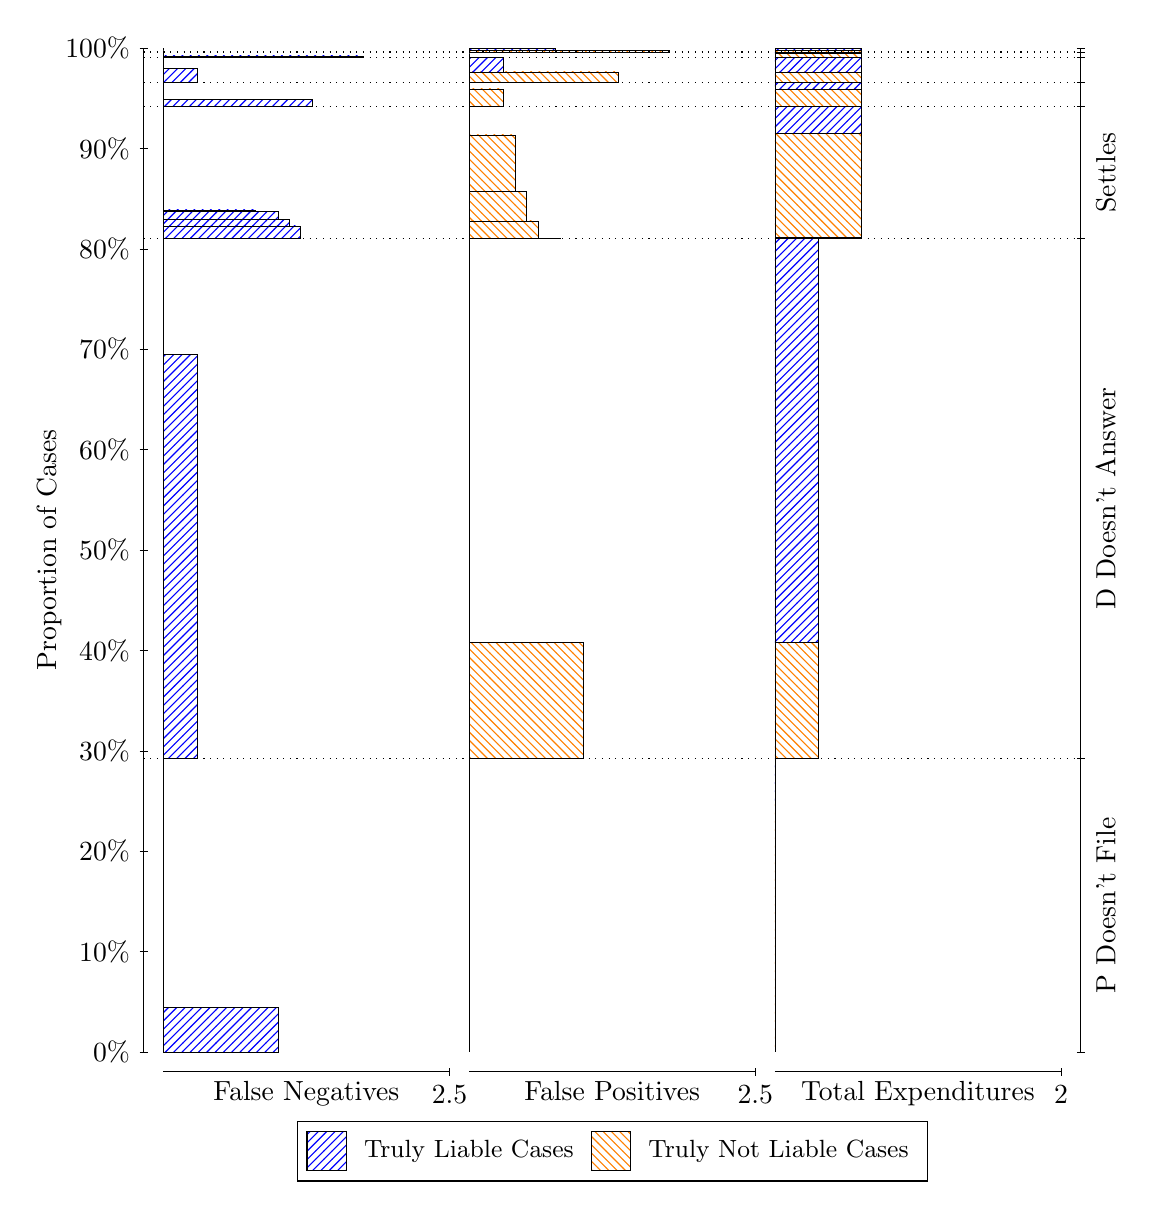
\begin{tikzpicture}
\draw[black, very thin] (1.5,1.75) -- (1.5,14.5);
\node[rotate=90, text=black, anchor=center] at (0.3, 8.125) {Proportion of Cases};
\draw[black, very thin] (1.45,1.75) -- (1.55,1.75);
\node[text=black, anchor=east] at (1.45, 1.75) {0\%};
\draw[black, very thin] (1.45,3.025) -- (1.55,3.025);
\node[text=black, anchor=east] at (1.45, 3.025) {10\%};
\draw[black, very thin] (1.45,4.3) -- (1.55,4.3);
\node[text=black, anchor=east] at (1.45, 4.3) {20\%};
\draw[black, very thin] (1.45,5.575) -- (1.55,5.575);
\node[text=black, anchor=east] at (1.45, 5.575) {30\%};
\draw[black, very thin] (1.45,6.85) -- (1.55,6.85);
\node[text=black, anchor=east] at (1.45, 6.85) {40\%};
\draw[black, very thin] (1.45,8.125) -- (1.55,8.125);
\node[text=black, anchor=east] at (1.45, 8.125) {50\%};
\draw[black, very thin] (1.45,9.4) -- (1.55,9.4);
\node[text=black, anchor=east] at (1.45, 9.4) {60\%};
\draw[black, very thin] (1.45,10.675) -- (1.55,10.675);
\node[text=black, anchor=east] at (1.45, 10.675) {70\%};
\draw[black, very thin] (1.45,11.95) -- (1.55,11.95);
\node[text=black, anchor=east] at (1.45, 11.95) {80\%};
\draw[black, very thin] (1.45,13.225) -- (1.55,13.225);
\node[text=black, anchor=east] at (1.45, 13.225) {90\%};
\draw[black, very thin] (1.45,14.5) -- (1.55,14.5);
\node[text=black, anchor=east] at (1.45, 14.5) {100\%};

\draw[black, very thin] (13.4,1.75) -- (13.4,14.5);
\draw[black, very thin] (13.35,1.75) -- (13.45,1.75);
\node[anchor=west] at (13.35, 1.75) {};
\draw[black, very thin] (13.35,5.4764) -- (13.45,5.4764);
\node[anchor=west] at (13.35, 5.4764) {};
\draw[black, very thin] (13.35,12.078) -- (13.45,12.078);
\node[anchor=west] at (13.35, 12.078) {};
\draw[black, very thin] (13.35,13.763) -- (13.45,13.763);
\node[anchor=west] at (13.35, 13.763) {};
\draw[black, very thin] (13.35,14.062) -- (13.45,14.062);
\node[anchor=west] at (13.35, 14.062) {};
\draw[black, very thin] (13.35,14.38) -- (13.45,14.38);
\node[anchor=west] at (13.35, 14.38) {};
\draw[black, very thin] (13.35,14.449) -- (13.45,14.449);
\node[anchor=west] at (13.35, 14.449) {};
\draw[black, very thin] (13.35,14.5) -- (13.45,14.5);
\node[anchor=west] at (13.35, 14.5) {};

\draw[black, very thin, pattern color=blue, pattern=north east lines] (1.75,1.75) rectangle (3.2033,2.312);
\draw[black, very thin, pattern color=orange, pattern=north west lines] (1.75,2.312) rectangle (1.75,5.4764);
\draw[black, very thin, pattern color=blue, pattern=north east lines] (1.75,5.4764) rectangle (2.186,10.607);
\draw[black, very thin, pattern color=orange, pattern=north west lines] (1.75,10.607) rectangle (1.75,12.078);
\draw[black, very thin, pattern color=blue, pattern=north east lines] (1.75,12.078) rectangle (3.494,12.241);
\draw[black, very thin, pattern color=blue, pattern=north east lines] (1.75,12.241) rectangle (3.3487,12.319);
\draw[black, very thin, pattern color=blue, pattern=north east lines] (1.75,12.319) rectangle (3.2033,12.429);
\draw[black, very thin, pattern color=blue, pattern=north east lines] (1.75,12.429) rectangle (2.9127,12.444);
\draw[black, very thin, pattern color=orange, pattern=north west lines] (1.75,12.444) rectangle (1.75,13.763);
\draw[black, very thin, pattern color=blue, pattern=north east lines] (1.75,13.763) rectangle (3.6393,13.843);
\draw[black, very thin, pattern color=orange, pattern=north west lines] (1.75,13.843) rectangle (1.75,14.062);
\draw[black, very thin, pattern color=blue, pattern=north east lines] (1.75,14.062) rectangle (2.186,14.246);
\draw[black, very thin, pattern color=orange, pattern=north west lines] (1.75,14.246) rectangle (1.75,14.38);
\draw[black, very thin, pattern color=blue, pattern=north east lines] (1.75,14.38) rectangle (4.2933,14.401);
\draw[black, very thin, pattern color=orange, pattern=north west lines] (1.75,14.401) rectangle (1.75,14.449);
\draw[black, very thin, pattern color=orange, pattern=north west lines] (1.75,14.449) rectangle (1.75,14.469);
\draw[black, very thin, pattern color=blue, pattern=north east lines] (1.75,14.469) rectangle (1.75,14.5);
\draw[black, very thin, pattern color=orange, pattern=north west lines] (5.6333,1.75) rectangle (5.6333,4.9144);
\draw[black, very thin, pattern color=blue, pattern=north east lines] (5.6333,4.9144) rectangle (5.6333,5.4764);
\draw[black, very thin, pattern color=orange, pattern=north west lines] (5.6333,5.4764) rectangle (7.0867,6.9468);
\draw[black, very thin, pattern color=blue, pattern=north east lines] (5.6333,6.9468) rectangle (5.6333,12.078);
\draw[black, very thin, pattern color=orange, pattern=north west lines] (5.6333,12.078) rectangle (6.796,12.085);
\draw[black, very thin, pattern color=orange, pattern=north west lines] (5.6333,12.085) rectangle (6.5053,12.306);
\draw[black, very thin, pattern color=orange, pattern=north west lines] (5.6333,12.306) rectangle (6.36,12.678);
\draw[black, very thin, pattern color=orange, pattern=north west lines] (5.6333,12.678) rectangle (6.2147,13.397);
\draw[black, very thin, pattern color=blue, pattern=north east lines] (5.6333,13.397) rectangle (5.6333,13.763);
\draw[black, very thin, pattern color=orange, pattern=north west lines] (5.6333,13.763) rectangle (6.0693,13.982);
\draw[black, very thin, pattern color=blue, pattern=north east lines] (5.6333,13.982) rectangle (5.6333,14.062);
\draw[black, very thin, pattern color=orange, pattern=north west lines] (5.6333,14.062) rectangle (7.5227,14.196);
\draw[black, very thin, pattern color=blue, pattern=north east lines] (5.6333,14.196) rectangle (6.0693,14.38);
\draw[black, very thin, pattern color=orange, pattern=north west lines] (5.6333,14.38) rectangle (5.6333,14.428);
\draw[black, very thin, pattern color=blue, pattern=north east lines] (5.6333,14.428) rectangle (5.6333,14.449);
\draw[black, very thin, pattern color=orange, pattern=north west lines] (5.6333,14.449) rectangle (8.1767,14.469);
\draw[black, very thin, pattern color=blue, pattern=north east lines] (5.6333,14.469) rectangle (6.7233,14.5);
\draw[black, very thin, pattern color=orange, pattern=north west lines] (9.5167,1.75) rectangle (9.5167,4.9144);
\draw[black, very thin, pattern color=blue, pattern=north east lines] (9.5167,4.9144) rectangle (9.5167,5.4764);
\draw[black, very thin, pattern color=orange, pattern=north west lines] (9.5167,5.4764) rectangle (10.062,6.9468);
\draw[black, very thin, pattern color=blue, pattern=north east lines] (9.5167,6.9468) rectangle (10.062,12.078);
\draw[black, very thin, pattern color=orange, pattern=north west lines] (9.5167,12.078) rectangle (10.607,12.085);
\draw[black, very thin, pattern color=blue, pattern=north east lines] (9.5167,12.085) rectangle (10.607,12.1);
\draw[black, very thin, pattern color=orange, pattern=north west lines] (9.5167,12.1) rectangle (10.607,13.412);
\draw[black, very thin, pattern color=blue, pattern=north east lines] (9.5167,13.412) rectangle (10.607,13.763);
\draw[black, very thin, pattern color=orange, pattern=north west lines] (9.5167,13.763) rectangle (10.607,13.982);
\draw[black, very thin, pattern color=blue, pattern=north east lines] (9.5167,13.982) rectangle (10.607,14.062);
\draw[black, very thin, pattern color=orange, pattern=north west lines] (9.5167,14.062) rectangle (10.607,14.196);
\draw[black, very thin, pattern color=blue, pattern=north east lines] (9.5167,14.196) rectangle (10.607,14.38);
\draw[black, very thin, pattern color=orange, pattern=north west lines] (9.5167,14.38) rectangle (10.607,14.428);
\draw[black, very thin, pattern color=blue, pattern=north east lines] (9.5167,14.428) rectangle (10.607,14.449);
\draw[black, very thin, pattern color=orange, pattern=north west lines] (9.5167,14.449) rectangle (10.607,14.469);
\draw[black, very thin, pattern color=blue, pattern=north east lines] (9.5167,14.469) rectangle (10.607,14.5);
\draw[black, dotted] (1.5,5.4764) -- (13.4,5.4764);
\draw[black, dotted] (1.5,12.078) -- (13.4,12.078);
\draw[black, dotted] (1.5,13.763) -- (13.4,13.763);
\draw[black, dotted] (1.5,14.062) -- (13.4,14.062);
\draw[black, dotted] (1.5,14.38) -- (13.4,14.38);
\draw[black, dotted] (1.5,14.449) -- (13.4,14.449);
\draw[black, very thin] (1.75,1.5) -- (5.3833,1.5);
\node[text=black, anchor=north] at (3.5667, 1.5) {False Negatives};
\draw[black, very thin] (5.3833,1.45) -- (5.3833,1.55);
\node[text=black, anchor=north] at (5.3833, 1.45) {2.5};

\draw[black, very thin] (5.6333,1.5) -- (9.2667,1.5);
\node[text=black, anchor=north] at (7.45, 1.5) {False Positives};
\draw[black, very thin] (9.2667,1.45) -- (9.2667,1.55);
\node[text=black, anchor=north] at (9.2667, 1.45) {2.5};

\draw[black, very thin] (9.5167,1.5) -- (13.15,1.5);
\node[text=black, anchor=north] at (11.333, 1.5) {Total Expenditures};
\draw[black, very thin] (13.15,1.45) -- (13.15,1.55);
\node[text=black, anchor=north] at (13.15, 1.45) {2};

\node[text=black, centered, rotate=90] at (13.72, 3.6132) {P Doesn't File};
\node[text=black, centered, rotate=90] at (13.72, 8.7771) {D Doesn't Answer};
\node[text=black, centered, rotate=90] at (13.72, 12.92) {Settles};





\draw (7.449999999999999,1.5) node[draw=none] (baseCoordinate) {};
\begin{scope}[align=center]
        \matrix[scale=0.5, draw=black, below=0.5cm of baseCoordinate, nodes={draw}, column sep=0.1cm]{
            \node[rectangle, draw, minimum width=0.5cm, minimum height=0.5cm, pattern color=blue, pattern=north east lines] {}; &
            \node[draw=none, font=\small, text=black] (B) {Truly Liable Cases}; &
            \node[rectangle, draw, minimum width=0.5cm, minimum height=0.5cm, pattern color=orange, pattern=north west lines] {}; &
            \node[draw=none, font=\small, text=black] (B) {Truly Not Liable Cases}; \\
            };
\end{scope}

\end{tikzpicture}
\end{document}